\chapter{ニューラルネットワーク}

本章では、Multilayer~perceptron及びその応用例のGenerative~Adversarial~Networksの説明を行った後、Generative~Adversarial~Networksを画像の変換に応用したPix2pixを紹介する。

\section{Multilayer~perceptron}

%Adam,SGDの原著論文に目を通す

Multilayer~perceptron~(MLP)~は複数のアフィン変換と非線形関数を合成した関数により定義され、式\ref{eq:MLP1}で定式化される。

\begin{align}
    \label{eq:MLP1}
    F_{MLP}(\boldsymbol{x})&=f_{n}(W_{n}(f_{n-1}(W_{n-1}\cdots(f_{1}(W_{1}\boldsymbol{x}+\boldsymbol{b_{1}}))\cdots+\boldsymbol{b_{n-1}}))+\boldsymbol{b_{n}})
\end{align}

ここで、$\boldsymbol{x}$は実ベクトル,$n$は1以上の整数,$f_{i}$は$i$番目の非線形関数,$W_{i}$は$i$番目の行列,$b_{i}$は$i$番目の実ベクトルである。また、MLPにおいては、$n$を層数、$W_i,b_i$を$i$番目の層の重み、と呼ぶ。

MLP~($F_{MLP}$)~を用いると、あるデータ集合$D=\{(\boldsymbol{x_j},\boldsymbol{t_j}); 1 \leqq j \leqq N\}$について、任意の$j$で$\boldsymbol{t_{j}}$の予測値として$\boldsymbol{y_j}=F_{MLP}(\boldsymbol{x_j})$を出力することができる。$\boldsymbol{t_j}$に近い$\boldsymbol{y_j}$を出力するためには、任意の$i$で$W_i,b_i$を適切に定める必要がある。

$y_j$と$t_j$の誤差を表す関数として損失関数$L(\boldsymbol{y_j},\boldsymbol{t_j})$を定義する。損失関数$L$を式\ref{eq:MLP2}に従って更新することで、$\boldsymbol{y_j}$を$\boldsymbol{t_j}$に近づける方向に層の重み$W_i,b_i$を更新することができる~(勾配降下法)~。

\begin{align}
    \label{eq:MLP2}
    W _i &\leftarrow W_i - \eta \frac{d L}{dW_i} \\
    b _i &\leftarrow b_i - \eta \frac{d L}{dW_i}
\end{align}

ここで、$\eta$は任意の正の実数であり、学習率と呼ばれる。なお、この学習率を適切に設定するためにStochastic~Gradient~Descent~\cite{SGD}やAdam~\cite{Adam}などのアルゴリズムが用いられる。

さらに、式\ref{eq:MLP3}で表される平均二乗誤差や式\ref{eq:MLP4}で表される平均絶対誤差などが損失関数として用いられる。

\begin{align}
    \label{eq:MLP3}
    L_{MSE}&=\frac{1}{n}\sum _{j=1} ^{n} {(\boldsymbol{y_j} - \boldsymbol{t_j})^2}\\
    \label{eq:MLP4}
    L_{MAE}&=\frac{1}{n}\sum _{j=1} ^{n} {|\boldsymbol{y_j} - \boldsymbol{t_j}|}
\end{align}

一般には、ニューラルネットワークはMLPより広い概念であるが、本論文ではこれ以降MLPのことをニューラルネットワークと呼ぶ。

\section{Generative~Adversarial~Networks}

\begin{figure}[t]
\begin{center}
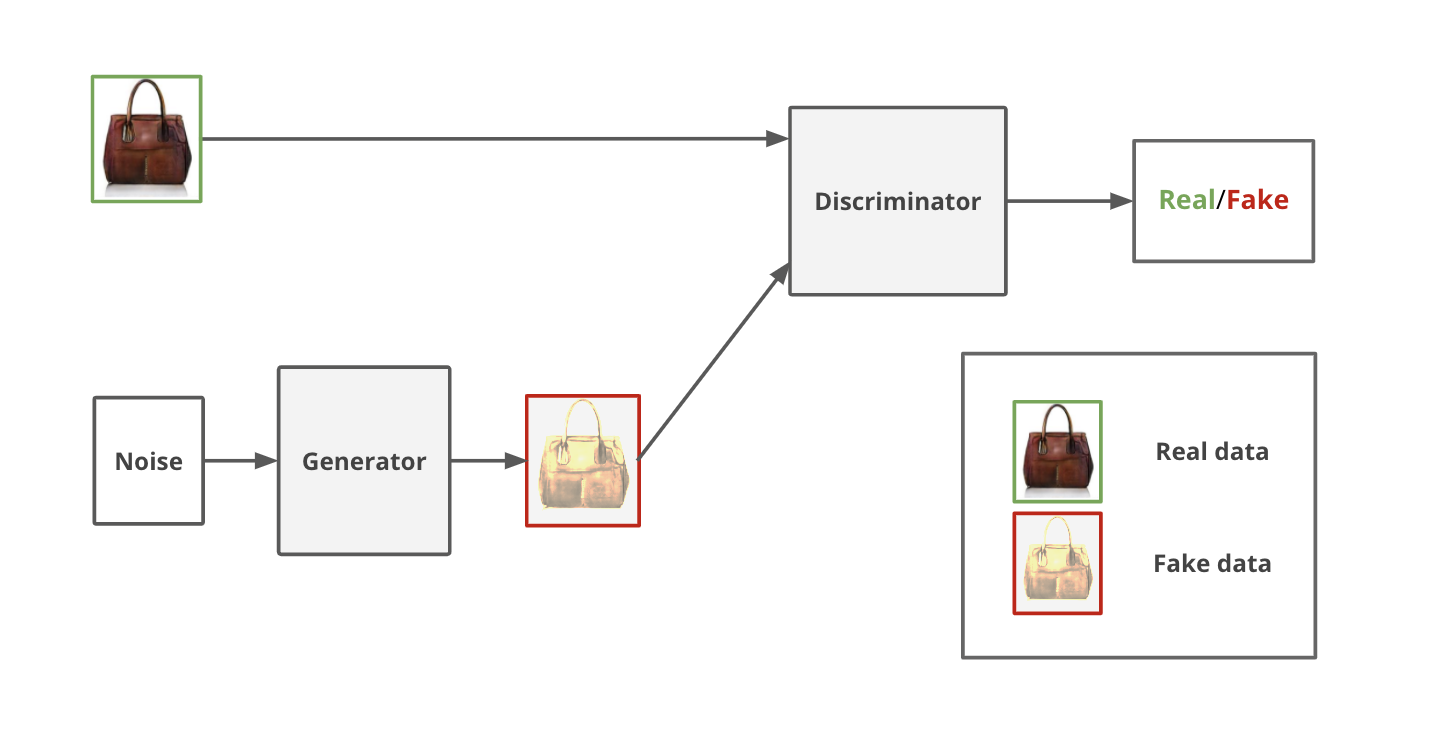
\includegraphics[width=\hsize]{figure/GAN_net.png}
\caption{GANのネットワーク、図は文献~\cite{pix2pix}のFigure~1を用いて作成。}
\label{fig:GAN_net}
\end{center}
\end{figure}

Generative~Adversarial~Networks~(GAN)~\cite{GAN}はニューラルネットワークの応用例であり、学習データの特徴を学習して擬似的なデータを生成することを目指す手法である。この手法は実在しないアイドルの写真を生成する際などに用いられる~\cite{idol}。

GANは図\ref{fig:GAN_net}のように二つのニューラルネットワークで構成される。それぞれのネットワークは~Discriminator~(識別モデル)~と~Generator~(生成モデル)~と呼ばれる。二つのネットワークはランダムに初期化された後に競合的に学習を進める。まず、識別モデルはデータが~Fake~data~(生成モデルの出力)~と~Real~data~(学習データ)~のどちらであるかを識別できるように学習を進める。そして、生成モデルは識別モデルが学習データであると誤って識別するように、~Noise~(ノイズ)~を元に学習データに近いデータを出力する。この二つの学習を交互に繰り返すことで、漸進的に生成モデルが学習データにより近いデータを生成できるようになると期待される。また、ノイズは適当な次元の実ベクトルであり、生成モデルの出力の揺らぎを表現する潜在変数の役割を果たす。

そして、GANにおいては、生成モデルの目的関数は式\ref{eq:GAN_G}、識別モデルの目的関数は式\ref{eq:GAN_D}として定式化される。

\begin{align}
    \label{eq:GAN_G}
    \argmin _{\theta_G}& \mathbb{E}_{\boldsymbol{z}}[\log (1-D(G(\boldsymbol{z};\theta_G);\theta_D))]\\
    \label{eq:GAN_D}
    \argmax _{\theta_D}& \mathbb{E}_{\boldsymbol{x}}[\log D(\boldsymbol{x};\theta_D)]+\mathbb{E}_{\boldsymbol{z}}[\log (1-D(G(\boldsymbol{z};\theta_G);\theta_D))]
\end{align}


ここで、$\boldsymbol{x}$は学習データ、$\boldsymbol{z}$は生成モデルへの入力のノイズ、$G(\boldsymbol{z};\theta_G)$はノイズ$\boldsymbol{z}$を入力とする生成モデル、$D(\cdot;\theta_D)$は識別モデル、$\theta_G$は生成モデル$G$のパラメータ、$\theta_D$は識別モデル$D$のパラメータ、である。

\section{Pix2pix}

\begin{figure}[t]
\begin{center}
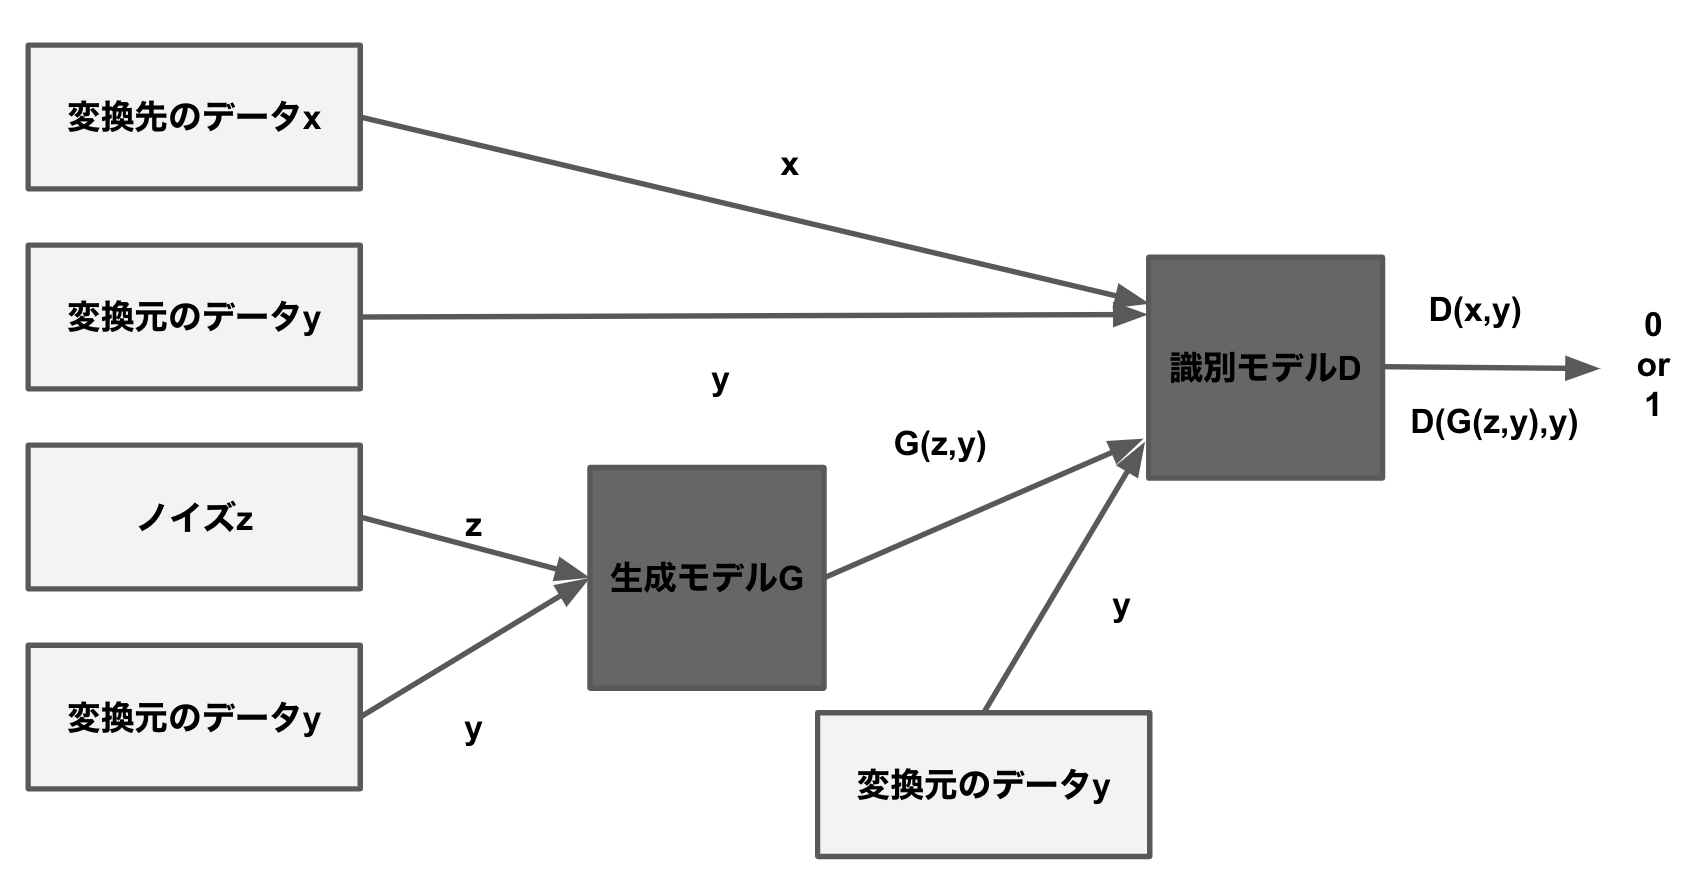
\includegraphics[width=\hsize]{figure/pix2pix_net.png}
\caption{pix2pixのネットワーク、図は文献~\cite{pix2pix}のFigure~1を用いて作成。}
\label{fig:pix2pix_net}
\end{center}
\end{figure}

\begin{figure}[t]
\begin{center}
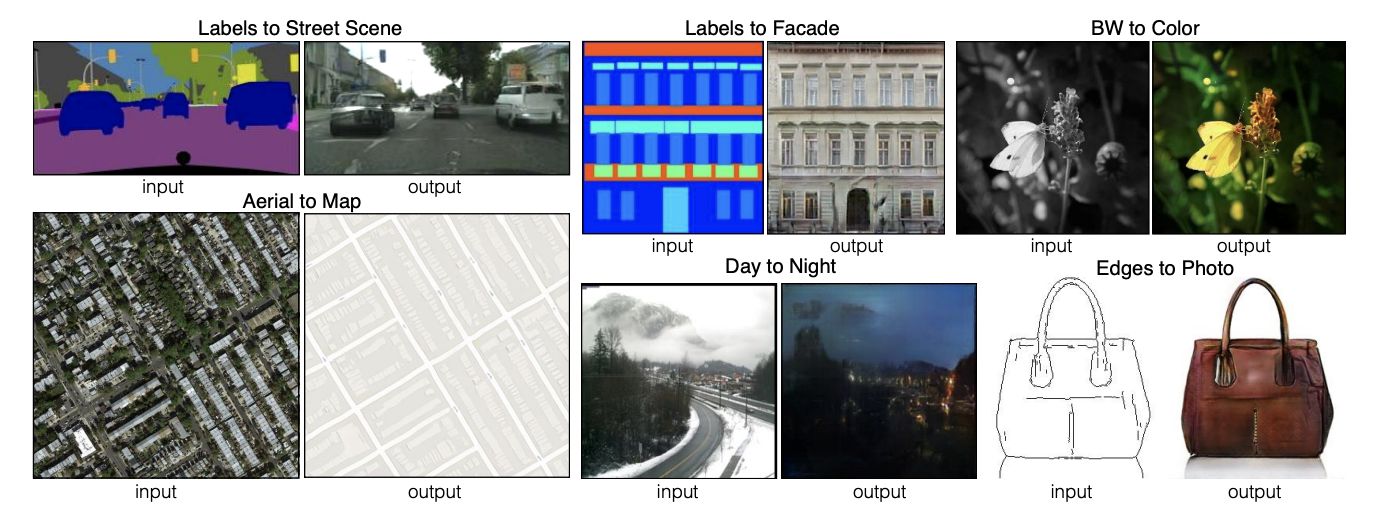
\includegraphics[width=\hsize]{figure/pix2pix_img.png}
\caption{pix2pixのスタイル変換の例、図は文献~\cite{pix2pix}のFigure~1を用いて作成。}
\label{fig:pix2pix_img}
\end{center}
\end{figure}

Pix2pix~\cite{pix2pix}は図\ref{fig:pix2pix_net}のようにネットワークの入力に変換元の画像を~Condition~(条件)~として与えることで画像の変換を行うGANである。特定の条件をネットワークの入力に与えるGANとしてはConditional~GAN~(CGAN)~\cite{CGAN}が初めて考案されたが、Pix2pixは与えられた条件画像の構造を維持したまま変換するという点でCGANとは異なる。具体的には、図\ref{fig:pix2pix_img}のように線画の写真への変換や白黒写真のカラー画像への変換を行うことができる。

そして、Pix2pixにおいては、生成モデルの目的関数は式\ref{eq:pix2pix_G}、識別モデルの目的関数は式\ref{eq:pix2pix_D}として定式化される。

\begin{align}
    \label{eq:pix2pix_G}
    \argmin _{\theta_G}& \mathbb{E}_{\boldsymbol{y}, \boldsymbol{z}}[\log (1-D(\boldsymbol{y}, G(\boldsymbol{y}, \boldsymbol{z}; \theta_G); \theta_D))]+\mathbb{E}_{\boldsymbol{x}, \boldsymbol{y}, \boldsymbol{z}}[\|\boldsymbol{x}-G(\boldsymbol{y}, \boldsymbol{z}; \theta_G)\|_{1}]\\
    \label{eq:pix2pix_D}
    \argmax _{\theta_D}& \mathbb{E}_{\boldsymbol{x}, \boldsymbol{y}}[\log D(\boldsymbol{x}, \boldsymbol{y}; \theta_D)]+\mathbb{E}_{\boldsymbol{y}, \boldsymbol{z}}[\log (1-D(\boldsymbol{y}, G(\boldsymbol{y}, \boldsymbol{z}; \theta_G); \theta_D))]
\end{align}

ここで、$\boldsymbol{x}$は変換先の学習データ、$\boldsymbol{y}$は変換元の学習データ、$\boldsymbol{z}$は生成モデルへの入力のノイズ、$G(\boldsymbol{y},\boldsymbol{z};\theta_G)$は$\boldsymbol{y}$を条件としノイズ$\boldsymbol{z}$を入力とする生成モデル、$D(\boldsymbol{y},\cdot;\theta_D)$は$\boldsymbol{y}$を条件とする識別モデル、$\theta_G$は生成モデル$G$のパラメータ、$\theta_D$は識別モデル$D$のパラメータ、である。

\subsection{生成モデルの構造}

\begin{figure}[t]
\begin{center}
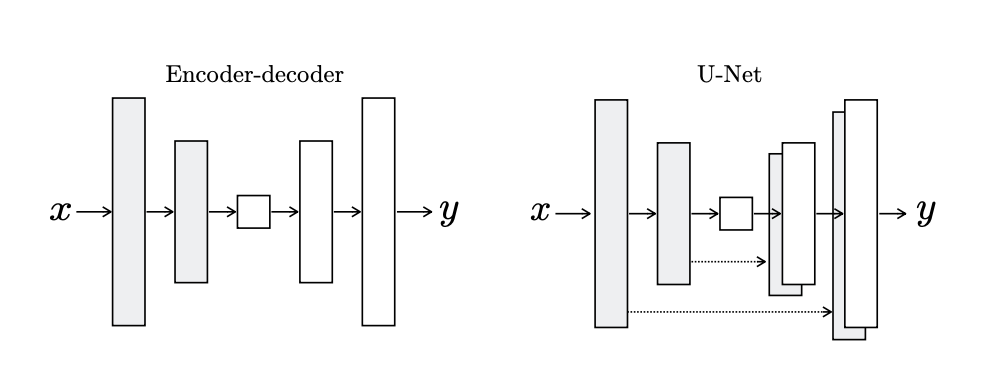
\includegraphics[width=\hsize]{figure/u-net.png}
\caption{生成モデルのネットワーク、図は文献~\cite{pix2pix}のFigure~1とFigure~3を用いて作成。}
\label{fig:u-net}
\end{center}
\end{figure}

Pix2pixの生成モデルには、図\ref{fig:u-net}のようにEncoder-Decoder型のネットワークが用いられる。ただし、変換元の画像とのピクセルの対応関係を維持するために、Skip~Connection~(スキップコネクション)~を持つ~\cite{u-net}。

また、ノイズとしては実ベクトルではなくDropoutが用いられる~\cite{Dropout}。Dropoutとは、ニューラルネットワークの重みの更新の際にランダムにいくつかの重みを0として無視する手法のことである。

\subsection{識別モデルの構造}

\begin{figure}[t]
\begin{center}
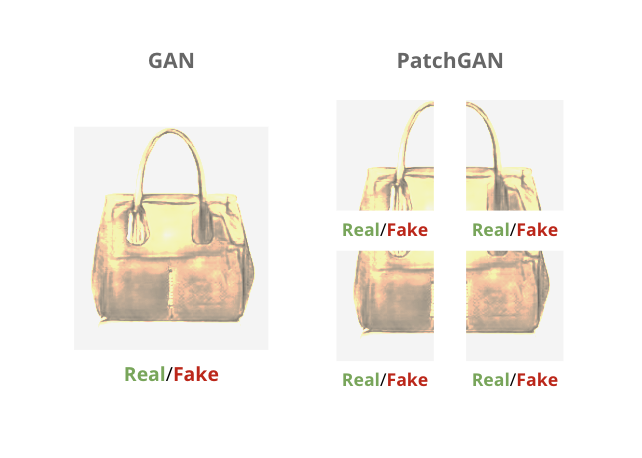
\includegraphics[width=\hsize]{figure/patchgan.png}
\caption{PatchGANの仕組み、図は文献~\cite{pix2pix}のFigure~1を用いて作成。}
\label{fig:patchgan}
\end{center}
\end{figure}

Pix2pixの識別モデルには、PatchGANという手法が用いられる。PatchGANは図\ref{fig:patchgan}のように画像全体ではなくパッチと呼ばれる小領域ごとに真偽を求めて平均を出力とする。これにより、局所的な識別精度が高まることが期待される。